\documentclass[runningheads]{llncs}
\usepackage[T1]{fontenc}
\usepackage{amsmath,amssymb,booktabs,graphicx,multirow}
\usepackage[hidelinks]{hyperref}
\setlength{\emergencystretch}{1.5em}
\begin{document}
\title{The Oracle Gap Has a Floor: Separating Aleatoric and Deployable Headroom in Evaluating Label Acquisition}
\titlerunning{The Oracle Gap Has a Floor}
\author{Anonymous Authors}
\authorrunning{Anonymous Authors}
\institute{Anonymous Institution}
\maketitle
\begin{abstract}
Oracle selectors in label-acquisition benchmarks can exploit both realized training outcomes and the evaluation set. We distinguish the value of perfect information about hidden training labels from test-set reuse and from the performance of a specified ex-ante selector. For a fixed feasible family, we derive distribution-free population inequalities and their exact empirical analogues; a Gaussian two-set expression is an approximation rather than a universal bound. Across 624 simulated states, the empirical inequalities hold throughout. Eight cohorts and three downstream learners reveal substantial variation in hindsight opportunity. Within-cohort label-flip interventions increase the empirical family floor monotonically in all three tested cohorts, while larger candidate pools show heterogeneous effects. Exact enumeration on 12-candidate pools checks a greedy-oracle approximation, and probability-model perturbations expose sensitivity beyond held-out calibration checks. We retain cross-fitted greedy performance as an operational benchmark, with its optimization and Monte Carlo errors stated explicitly. Delayed replay shows that DC-PRISM can improve on quantity-oriented references while losing to information-greedy rules. The resulting protocol audits which parts of an oracle gap are supported by an evaluation design, rather than treating the entire gap as attainable improvement.
\keywords{Active learning \and Evaluation \and Oracle bounds \and Aleatoric uncertainty \and Risk-constrained acquisition}
\end{abstract}

\section{Introduction}
\label{sec:intro}
How much better could an acquisition strategy be? Active-learning research increasingly answers with an \emph{oracle}: a selector that, unlike any deployable strategy, may look at the labels it acquires and at the evaluation set, and so traces the best attainable learning curve. Recent benchmarks construct greedy oracles that add, step by step, the candidate whose \emph{realized} label most improves test performance~\cite{werner2023comparable,werner2024cdalbench}, and best-of-strategies oracles that pick, per batch, the strategy whose labelled batch helps most~\cite{huseljic2026boss}. The gap between oracle and practical strategies is then read as headroom: state-of-the-art strategies are reported to ``fall noticeably short of oracle performance, especially in large-scale datasets''~\cite{huseljic2026boss}. This complements a broader effort to make active-learning evaluation reliable~\cite{luth2023navigating,ji2023randomness}.

An oracle that selects with realized labels is an \emph{ex-post} benchmark. Part of its advantage is unreachable by construction: when outcomes are random given the covariates, some feasible label set will turn out to be lucky, and only hindsight can find it. The distinction between ex-post and ex-ante regret is familiar in decision-focused learning and robust optimization~\cite{schutte2023robust}, and in bandits the gap between expected regret and pseudo-regret grows with the noise of the arms~\cite{bubeck2012regret,audibert2010regret}. We investigate its magnitude for oracle bounds in label acquisition, where it affects whether an ``oracle gap'' signals room for better strategies or merely outcome noise. Labels in credit, healthcare and marketing record stochastic outcomes rather than near-deterministic categories, so the question matters most where labels are bought with consequential actions.

\paragraph{Contributions.}
\begin{itemize}
\item A protocol distinguishing fixed-family perfect-information value, evaluation-set reuse, and the gain of a specified cross-fitted selector. These quantities have different identification and estimation requirements.
\item Distribution-free inequalities for the fixed-family floor, checked on 624 states, together with exact small-pool enumeration, probability-model sensitivity, and within-cohort label-noise interventions.
\item An empirical audit across eight cohorts and three learners, with delayed replay as a separate outcome check. The evidence documents where hindsight opportunity persists and where practical selection rules fail to exploit it.
\end{itemize}



\section{Setting}
\label{sec:setting}
At round $t$ a learner holds labeled history $D_t$, the covariates of pending acquisitions $O_t$ (selected but not yet resolved), an unlabeled candidate pool $C_t$ and target covariates $Q_t$. Candidate $i$ has a visible exposure $e_i\ge0$ and a binary outcome $Y_i$ revealed only after acquisition. A strategy chooses $S_t\subseteq C_t$ from visible information $\mathcal H_t$. Learning is measured by the Brier score~\cite{brier1950verification} of a downstream learner (an $\ell_2$-logistic model, gradient boosting, or a one-hidden-layer network); $L(S;Y)$ is its test loss after fitting on $D\cup O\cup S$, where $Y$ collects the hidden training outcomes of $O$ and $S$.

\paragraph{Risk budget.} Acquiring a label is an action with exposure, as when a lender approves an applicant to observe repayment~\cite{lakkaraju2017selective,wei2021selective}. With a risk score $q_i$, $\ell=\log(1/\alpha)$ and $\phi(q)=q(1-q)$ for $q\le\frac12$, $\frac14$ otherwise, feasible sets satisfy
\begin{equation}
 R_\alpha(S)=\sum_{i\in S}e_iq_i+\Big(2\ell\sum_{i\in S}e_i^2\phi(q_i)\Big)^{1/2}+\frac{\ell}{3}\max_{i\in S}e_i\le B_t,
 \label{eq:envelope}
\end{equation}
a sub-gamma bound~\cite{boucheron2013concentration} under which realized adverse exposure exceeds $R_\alpha(S)$ with probability at most $\alpha=0.1$ under conditional independence and $p_i\le q_i$. Our scores $q_i$ (a Wilson-shifted~\cite{wilson1927probable} high quantile of 40 Laplace draws of the fitted logit) do not guarantee $p_i\le q_i$, so~\eqref{eq:envelope} is the operational feasible region shared by all strategies. The budget $B_t$ is $1.03$ times the envelope of the $k$ lowest-risk candidates ($k=6$ unless stated); the \emph{quantity reference} $M_K$ is the largest feasible set, found by enumeration for at most 16 candidates and otherwise by an exposure-stratified search that certified its cardinality in 1{,}320 of 1{,}408 states ; exact follow-up search certified all remaining 88 reference counts. For benchmark cohorts without a natural exposure we set $e_i=1$.

\section{Decomposing the Oracle Gap}
\label{sec:protocol}
\paragraph{Family oracle.} Fix $\mathcal H$ and a family $\mathcal F$ of feasible sets built from visible information and containing $M=M_K$. With $\bar L$ the test loss with test-label noise integrated out,
\begin{align}
 H_{\mathrm{post}}&=\mathbb E\big[\bar L(M;Y)-\min_{S\in\mathcal F}\bar L(S;Y)\mid\mathcal H\big],\\
 H_{\mathrm{pre}}&=\mathbb E[\bar L(M;Y)\mid\mathcal H]-\min_{S\in\mathcal F}\mathbb E[\bar L(S;Y)\mid\mathcal H].
\end{align}
$H_{\mathrm{post}}$ is the lead of an oracle that picks the best set after seeing the hidden training labels; $H_{\mathrm{pre}}$ is the lead of the best fixed choice. Their difference, the \emph{aleatoric floor} $F=H_{\mathrm{post}}-H_{\mathrm{pre}}\ge0$ (since $\mathbb E\min\le\min\mathbb E$), is unreachable by any strategy restricted to $\mathcal F$; it is the expected value of perfect information about the training outcomes~\cite{howard1966information}. For a within-family strategy with expected gain $\Gamma_\pi$ over $M$, $H_{\mathrm{post}}-\Gamma_\pi=F+(H_{\mathrm{pre}}-\Gamma_\pi)$, and only the second term, the \emph{selection gap}, can be closed.

\paragraph{Greedy benchmark diagnostics.} Benchmarks select a batch greedily using realized labels and an evaluation set~\cite{werner2023comparable,werner2024cdalbench}. We split test records into $T_1,T_2$. Let $G_{\rm rep}$ be the greedy selector's mean gain when selecting and scoring on $T_1$, $G_{\rm hold}$ its gain when scoring on $T_2$, and $G_{\rm cf}$ the gain of a greedy selector choosing by mean $T_1$ loss on one bank of training-label replicates and evaluated on $T_2$ using an independent bank, with banks exchanged and averaged. Then
\[
G_{\rm rep}=(G_{\rm rep}-G_{\rm hold})+(G_{\rm hold}-G_{\rm cf})+G_{\rm cf}.
\]
This is an accounting identity. The first contrast diagnoses evaluation-set reuse; the second is a \emph{greedy residual}, which also contains search and finite-simulation effects. It equals the fixed-family floor only when the respective selectors optimize a common family and their objectives and evaluation distributions agree. We therefore do not identify this residual as an irreducible floor or call $G_{\rm cf}$ the optimal deployable value.

\paragraph{Valid fixed-family inequalities.} Write $d_S=\bar L(M;Y)-\bar L(S;Y)$, $\mu_S=\mathbb E d_S$, and let $b$ maximize $\mu_S$; let $r$ be another set. The family floor is $F=\mathbb E\max_S d_S-\max_S\mu_S$. Pointwise comparison with $b,r$, and centering each gain, give
\begin{equation}
\mathbb E(d_r-d_b)_+\ \leq F\ \leq\mathbb E\max_S(d_S-\mu_S).\label{eq:two}
\end{equation}
Indeed, $\max_S d_S-d_b\ge(d_r-d_b)_+$, whereas $\max_S d_S\le\max_S\mu_S+\max_S(d_S-\mu_S)$. Replacing expectations and means by the same empirical distribution gives exact sample inequalities, including when $b,r$ are selected from that sample. These empirical statements do not provide confidence coverage for population $F$. If the centered gains are jointly Gaussian, arbitrary dependence is allowed and $F\le\max_S\sigma_S\sqrt{2\log|\mathcal F|}$. If $d_b-d_r$ is normal with mean $\Delta$ and standard deviation $s$, the lower expression is $s\varphi(\Delta/s)-\Delta\Phi(-\Delta/s)$. Normality is an additional modeling assumption. An independent-normal construction is not a universal upper bound.

\paragraph{Estimation and model substitution.} With known $p$, common random numbers generate training-label replicates. For a fixed family, maximizing estimated mean gain gives an upward-biased estimate of $H_{\rm pre}$ in expectation. Selecting on one label bank and evaluating on another yields the expected value of that finite-bank selector, at most $H_{\rm pre}$. Neither expectation statement is a deterministic finite-sample bracket. On real data, a boosting model fitted on disjoint auxiliary records supplies $\hat p$; recorded test labels remain fixed. This evaluates opportunity conditional on that test set and probability model. Comparing simulated and recorded-outcome hindsight gaps tests one functional of the model, not full identification of the floor. Taking the per-state maximum of independently noisy policy-value estimates can itself introduce selection optimism; such post-hoc maxima are sensitivity summaries, not certified lower bounds on achievable value.

\section{Strategies under Evaluation}
\label{sec:policy}
All strategies share the state, $q$, the budget and~\eqref{eq:envelope}. \emph{Safe-MinRisk} returns $M_K$; \emph{fixed count} takes a fixed fraction of $K$ by point value; \emph{Fisher-cost} packs by single-label variance reduction per exposure. Four rules pack greedily until no feasible candidate remains: \emph{Random}, \emph{Uncertainty}~\cite{lewis1994sequential}, \emph{BAIT-greedy} on $\operatorname{tr}(F_Q(H_{D+O}+A_S)^{-1})$~\cite{ash2021fishing}, and \emph{TargetVar-greedy} on the target-weighted proxy
\begin{equation}
 V_\theta(S)=\operatorname{tr}\big[W_Q\{H_{D+O}^{-1}-(H_{D+O}+A_S)^{-1}\}\big],\label{eq:value}
\end{equation}
where $H_{D+O}$ is the logistic Fisher information of history and pending covariates, $A_S$ that of $S$, and $W_Q$ weights target directions by their Brier sensitivity~\cite{yu2006transductive,bickfordsmith2023prediction}. \emph{Proxy-argmax} picks $\arg\max V_{\hat\theta}$ over the evaluation family. \emph{DC-PRISM} is a conservative policy designed for risk-constrained acquisition with pending outcomes: it evaluates~\eqref{eq:value} on a family anchored at $M_K$ under 20 Laplace parameter draws~\cite{mackay1992practical}, scores each set by the 0.2-quantile of $\tanh\{(V_m(S)-V_m(M_K))/2.5V_m(M_K)\}$ minus a quantity penalty $0.22(K-|S|)_+/K$, and returns $M_K$ unless the best score exceeds $0.08$. A selection takes about 50\,ms with 24 candidates. All information proxies here are derived from the logistic model.

\section{Validating the Protocol}
\label{sec:validation}
\paragraph{Studies.} Every study fixed its states, seeds, comparison families and a material-effect threshold of $5\times10^{-4}$ Brier before running, with protocol and code frozen in version control; we report paired means with 95\% Bonferroni simultaneous intervals and Holm-adjusted tests~\cite{holm1979simple}. All values are in $10^{-3}$ Brier. Cohorts: four credit cohorts (HMEQ, LendingClub, PPDai, UCI Credit~\cite{sasHMEQ,lendingclubSource,ppdaiSource,he2018ensemble,yeh2009comparison}), 30-day hospital readmission~\cite{strack2014impact} with days in hospital as exposure, bank-marketing subscription, Spambase, and USPS digits ($\ge5$ versus $<5$), the last as raw pixels and as 10 principal components. Each state is the first round of a delayed replay with 68 historical labels, 14 pending and 24 candidate records; candidates are drawn at random (\emph{natural} stream) or, for credit and readmission, also from an \emph{engineered} stream that ranks covariates into low-risk, pending-aligned, complementary and tail candidates. Controlled worlds and \emph{semi-synthetic} states (real covariates, outcomes from a known logit) provide known $p$.

\paragraph{Estimated probabilities recover known-probability values.} On 512 semi-synthetic states, boosting $\hat p$ fitted on auxiliary records labeled from the true $p$ gives estimates whose bias against the known-$p$ protocol lies within $\pm0.5$ in 95 of 96 checks (8 groups $\times$ 12 quantities); mean biases of $H_{\mathrm{post}}$, $H_{\mathrm{pre}}$, the floor and the main strategy gains are at most $0.20$, with state-level correlations of $0.73$--$0.95$ for $H_{\mathrm{pre}}$. A logistic $\hat p$ underestimates $H_{\mathrm{pre}}$ by $0.26$--$0.28$ where the truth is nonlinear, so the estimator needs a flexible $\hat p$.

\paragraph{Recorded-outcome checks and sensitivity.} A confidence interval containing zero does not establish agreement. In the revision we use equivalence tests with margin $0.5$ in the displayed units. Pooled checks for logistic and boosting learners support equivalence, while only two of 16 individual cohort--learner cells establish it; the neural learner does not establish pooled equivalence. In 192 additional greedy-calibration states, the pooled reported-gap difference has 90\% interval $[-0.089,0.416]$, within the margin, whereas the held-out-gap interval $[-0.138,0.513]$ crosses it. Known-probability perturbations give mean floor bias about $-0.04$ at the unperturbed model, but changing probability sharpness shifts bias by approximately $0.5$--$0.8$. Disjoint fitting is essential but does not establish robustness to probability-model misspecification.

\paragraph{Family sensitivity.} Enlarging each family with 64 random feasible sets (from 22--27 to 81--88 sets) in these experiments leaves the estimated deployable share $H_{\mathrm{pre}}/H_{\mathrm{post}}$ essentially unchanged: 80--83\% in controlled worlds at every sub-family size from 2 to 80, and 6--38\% on semi-synthetic arms, where it rises slightly rather than falls with $|\mathcal F|$.

\section{Findings}
\label{sec:findings}
\paragraph{The greedy benchmark gap shrinks under held-out selection.} Table~\ref{tab:known} retains the original cross-fitted greedy estimates. Its columns implement the accounting identity in Section~\ref{sec:protocol}; the residual column includes approximation error and is not the fixed-family $F$. On semi-synthetic states the reported lead over the best fixed strategy is $6.9$, while the cross-fitted greedy lead is approximately zero. On recorded-outcome states, correction reduces the apparent lead substantially. This demonstrates sensitivity to evaluation design, without proving that the entire removed component is irreducible.

\begin{table}[t]
\caption{Benchmark greedy oracle under the risk budget, logistic learner ($\times10^{-3}$ Brier). Reported gap $=$ test reuse $+$ greedy residual $+$ cross-fitted greedy gain. Last column: lead over the best fixed practical strategy, as reported $\to$ after removing reuse and floor.}
\label{tab:known}
\centering\scriptsize
\setlength{\tabcolsep}{3.5pt}
\begin{tabular}{lrrrrrr}
\toprule
Setting & States & Reported & Reuse & Residual & CF greedy & Lead over best \\
\midrule
Controlled worlds & 64 & 29.5 & 4.5 & 3.5 & 21.5 & 15.8$\to$7.8 \\
Semi-synthetic (known $p$) & 256 & 7.2 & 2.9 & 3.9 & 0.3 & 6.9$\to$0.0 \\
Credit, engineered stream & 128 & 8.0 & 0.6 & 4.1 & 3.3 & 6.7$\to$2.0 \\
Credit, natural stream & 128 & 3.4 & 0.8 & 1.7 & 0.9 & 3.2$\to$0.6 \\
Readmission, both streams & 64 & 2.3 & 0.3 & 1.4 & 0.5 & 2.0$\to$0.3 \\
\bottomrule
\end{tabular}
\end{table}

\paragraph{Noise ordering and a direct intervention.} The original cross-cohort study registered a relationship between the noise index and the greedy residual share (Table~\ref{tab:gradient}). Its interpretation depends on the ex-ante comparator: using a post-hoc strengthened comparator changes the logistic rank correlation to $0.93$ and the neural correlation to $0.52$ ($p=0.15$). The latter no longer supplies clear cross-cohort evidence. A distinct registered intervention flips labels with probability $0,0.1,0.2,0.3$ within HMEQ, Bank Marketing and USPS, using 16 states per dose and cohort. The empirical fixed-family floor increases monotonically in all three cohorts (Figure~\ref{fig:floor}b). This intervention supports a response to randomized label corruption within the specified simulation; it does not establish a universal monotonic relationship for natural label noise.

\begin{table}[t]
\caption{Benchmark oracle along a label-noise gradient (natural stream, 48 states per cohort with the logistic and 32 with the neural learner; $\times10^{-3}$ Brier). Noise: mean $\hat p(1-\hat p)$. Reuse and floor: \% of the reported gap. Lead: over the best fixed strategy, reported $\to$ deployable.}
\label{tab:gradient}
\centering\scriptsize
\setlength{\tabcolsep}{2.6pt}
\begin{tabular}{lrrrrrrrrr}
\toprule
& & \multicolumn{4}{c}{Logistic learner} & \multicolumn{4}{c}{Neural learner (MLP)} \\
\cmidrule(lr){3-6}\cmidrule(lr){7-10}
Cohort & Noise & Gap & Reuse & Residual & Lead & Gap & Reuse & Residual & Lead \\
\midrule
USPS, raw pixels & 0.036 & \multicolumn{4}{c}{--} & 18.7 & 32 & 10 & 15.9$\to$8.0 \\
Spambase & 0.054 & 7.5 & 32 & 16 & 5.1$\to$1.5 & 14.1 & 25 & 29 & 11.4$\to$3.8 \\
USPS, 10 PCs & 0.065 & 10.8 & 12 & 13 & 7.7$\to$5.0 & 16.6 & 23 & 29 & 15.0$\to$6.4 \\
Readmission & 0.081 & 1.3 & 29 & 66 & 1.1$\to$$-$0.1 & 4.8 & 23 & 54 & 4.0$\to$0.3 \\
Bank Marketing & 0.091 & 4.5 & 15 & 39 & 4.1$\to$1.7 & 11.9 & 34 & 29 & 10.3$\to$2.8 \\
HMEQ & 0.101 & 3.4 & 15 & 42 & 3.0$\to$1.0 & 7.8 & 26 & 39 & 7.2$\to$2.1 \\
PPDai & 0.108 & 2.8 & 17 & 60 & 2.7$\to$0.5 & 10.4 & 20 & 38 & 9.1$\to$3.0 \\
UCI Credit & 0.136 & 3.4 & 15 & 67 & 3.2$\to$0.4 & 8.2 & 47 & 38 & 7.8$\to$0.8 \\
LendingClub & 0.144 & 2.7 & 8 & 79 & 2.8$\to$0.4 & 8.5 & 39 & 53 & 8.6$\to$0.7 \\
\bottomrule
\end{tabular}
\end{table}

\paragraph{Bounds, search, and scale checks.} The corrected empirical lower and upper inequalities hold in all 624 revision states. Their validity is algebraic; this check verifies implementation, not a new population confidence guarantee. Stress tests with negative dependence, skewness and heavy tails invalidate the former independent-normal shortcut. In 12-candidate pools, exact enumeration of all feasible sets (about 730 on average) yields similar aggregate greedy diagnostics: the mean residual difference is approximately $-0.02$ and the ex-ante gain difference $0.01$ in displayed units. This checks approximation at that scale. Candidate pools of 24, 48 and 96 produce heterogeneous floor changes, so no large-pool approximation guarantee follows.

\begin{figure}[t]
\centering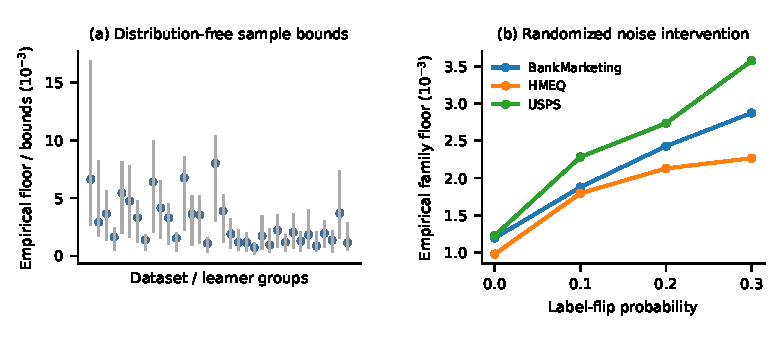
\includegraphics[width=\linewidth]{figures/fig_predict.pdf}
\caption{Corrected diagnostics. (a) Empirical lower bound, floor and upper bound by group, covering 624 states; this verifies the empirical identity, not population coverage. (b) Within-cohort randomized label flips: empirical family floor at four doses, 16 states per dose and cohort. Lines connect descriptive means.}
\label{fig:floor}
\end{figure}

\paragraph{Budget sensitivity is empirical.} Increasing a budget can enlarge a feasible family, but $F=H_{\rm post}-H_{\rm pre}$ is a difference of two changing quantities and need not increase. In the registered budget experiment, varying the target count from 3 to 6 to 12 increased the measured family floor in all eight cohorts, with paired mean increase $0.74$ $[0.67,0.82]$ in displayed units (Figure~\ref{fig:budget}). This is a result for the tested distributions and learner, rather than a consequence of~\eqref{eq:two}.

\begin{figure}[t]
 \centering
 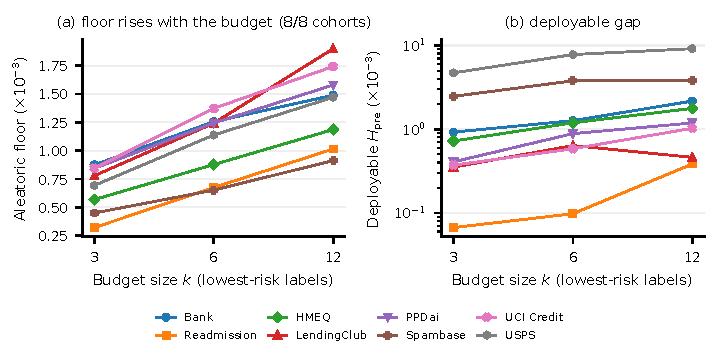
\includegraphics[width=\linewidth]{figures/fig_budget.pdf}
 \caption{Risk budget as a lever (logistic learner, 32 states per cohort and budget). The budget is sized for the $k$ lowest-risk candidates. (a) The aleatoric floor rises monotonically in all eight cohorts. (b) The deployable gap (log scale) moves much less uniformly.}
 \label{fig:budget}
\end{figure}

\paragraph{Who closes the estimated ex-ante selector gain depends on the learner.} Table~\ref{tab:who} reports, on the same real-label states, the estimated ex-ante selector gain and the gains of three strategies under two learners. With the logistic learner, information proxies derived from that model close a large part of it where it is largest: on engineered HMEQ and LendingClub TargetVar-greedy and Proxy-argmax capture $1.5$--$2.1$ of $3.2$--$3.4$ (in an independent 128-seed batch, $2.5$--$2.9$ of $4.9$--$5.7$, while DC-PRISM trails TargetVar-greedy by $2.8$ $[0.0,5.6]$ on LendingClub). With the boosting learner the estimated ex-ante selector gain is still $0.7$--$2.7$, DC-PRISM's selection gap is material in six of eight credit cells, and no strategy captures more than $0.65$: proxies that match the logistic model do not transfer to the boosting learner. On readmission the estimated ex-ante selector gain is small ($0.7$--$0.9$) and no strategy differs decisively.

\begin{table}[t]
\caption{Cross-fitted finite-family selector gain and gains over $M_K$ on real-label states (64 credit and 128 readmission states per cell; $\times10^{-3}$ Brier). DC: DC-PRISM; TV: TargetVar-greedy; Proxy: Proxy-argmax.}
\label{tab:who}
\centering\scriptsize
\setlength{\tabcolsep}{3pt}
\begin{tabular}{lrrrrrrrr}
\toprule
& \multicolumn{4}{c}{Logistic learner} & \multicolumn{4}{c}{Boosting learner} \\
\cmidrule(lr){2-5}\cmidrule(lr){6-9}
State & CF gain & DC & TV & Proxy & CF gain & DC & TV & Proxy \\
\midrule
HMEQ, eng. & 3.21 & 0.09 & 1.51 & 1.64 & 2.32 & 0.48 & 0.15 & 0.44 \\
LC, eng. & 3.37 & 1.15 & 2.01 & 2.12 & 1.53 & 0.05 & $-$0.42 & $-$0.19 \\
PPDai, eng. & 1.87 & 0.37 & 0.04 & 0.07 & 1.18 & 0.33 & 0.17 & 0.11 \\
UCI, eng. & 0.16 & $-$0.08 & $-$0.08 & $-$0.08 & 0.84 & 0.36 & 0.42 & 0.34 \\
HMEQ, nat. & 1.26 & $-$0.22 & 0.21 & 0.12 & 2.66 & 0.24 & 0.64 & 0.65 \\
LC, nat. & 0.91 & $-$0.04 & $-$0.20 & $-$0.05 & 1.45 & $-$0.07 & 0.04 & $-$0.04 \\
PPDai, nat. & 0.59 & 0.10 & $-$0.17 & 0.02 & 1.17 & $-$0.03 & $-$0.18 & $-$0.10 \\
UCI, nat. & 0.92 & 0.07 & 0.19 & 0.32 & 1.60 & 0.03 & 0.13 & 0.08 \\
Readm., eng. & 0.84 & 0.09 & $-$0.14 & $-$0.34 & 0.92 & $-$0.01 & $-$0.25 & $-$0.28 \\
Readm., nat. & 0.67 & 0.06 & 0.30 & 0.36 & 0.72 & 0.00 & $-$0.10 & $-$0.07 \\
\bottomrule
\end{tabular}
\end{table}

\paragraph{DC-PRISM in controlled worlds.} In worlds built around directional pending information, 83\% of hindsight headroom is estimated as ex-ante value and DC-PRISM captures two thirds of it: its gain over Safe-MinRisk is $12.2$ $[7.6,16.8]$ with $3.1$ instead of 6 labels, and remains material in all twelve generator variants we tried ($10.8$--$31.4$; pending overlap, risk--information coupling, no misspecified tail, 48 candidates with $K=12$). A common-family ablation attributes this gain to the proxy evaluated over an anchored family (Proxy-argmax alone gains $13.1$ $[6.1,20.2]$); the conservative layer adds an unconfirmed $3.0$ $[-0.2,6.2]$, and pending-awareness is not isolated by our evidence.

\section{Outcome Check: Delayed Replay}
\label{sec:replay}
The protocol scores single rounds. To check its ordering under dynamics we replayed ten rounds (exploration labels after one round, ordinary labels after two; ALC-Brier averages ten round-start scores) with 512 fresh seeds per credit cell and 256 per readmission stream, numbers registered from the variance of an earlier batch. Table~\ref{tab:replay} reports a separate dynamic comparison. Where information-greedy rules captured the deployable gap and DC-PRISM did not (engineered HMEQ and LendingClub), DC-PRISM is materially worse than Fisher-cost, BAIT-greedy and TargetVar-greedy ($2.5$--$3.8$); where its gain over the quantity reference was significant, it beats Safe-MinRisk and fixed count ($2.2$--$3.1$); on engineered readmission it beats BAIT-greedy and TargetVar-greedy ($1.3$, $1.4$); and where little deployable gap exists (natural streams, engineered UCI) no comparison is material. Realized adverse exposure exceeded the envelope in 0--4 of 40{,}960 acquisition rounds per credit policy and in none of 5{,}120 for readmission.

\begin{table}[t]
\caption{Delayed replay: comparator minus DC-PRISM ALC-Brier ($\times10^{-3}$; positive favors DC-PRISM; bold: material under the registered family).}
\label{tab:replay}
\centering\scriptsize
\setlength{\tabcolsep}{2.4pt}
\begin{tabular}{lrrrrrrrrrr}
\toprule
& \multicolumn{4}{c}{Credit, engineered} & \multicolumn{4}{c}{Credit, natural} & \multicolumn{2}{c}{Readmission} \\
\cmidrule(lr){2-5}\cmidrule(lr){6-9}\cmidrule(lr){10-11}
Comparator & HMEQ & LC & PPDai & UCI & HMEQ & LC & PPDai & UCI & eng. & nat. \\
\midrule
Safe-MinRisk & \textbf{2.4} & 0.4 & \textbf{3.1} & $-$0.1 & 0.2 & 0.2 & 0.4 & 0.1 & 0.0 & 0.2 \\
Fixed count & \textbf{2.2} & 0.4 & \textbf{2.4} & $-$0.1 & 0.1 & 0.1 & 0.3 & 0.0 & 0.4 & 0.2 \\
Random & 0.6 & $-$0.3 & \textbf{2.4} & 0.0 & 0.3 & 0.5 & 0.6 & 0.4 & 0.8 & 0.5 \\
Uncertainty & 0.5 & 1.4 & 0.7 & 0.0 & 0.4 & 0.4 & 0.1 & 0.1 & 0.4 & 0.0 \\
Fisher-cost & \textbf{$-$3.8} & \textbf{$-$3.3} & 0.8 & $-$0.1 & $-$0.3 & $-$0.1 & 0.1 & $-$0.1 & 1.0 & 0.0 \\
BAIT-greedy & \textbf{$-$3.6} & \textbf{$-$2.7} & 0.3 & 0.1 & $-$0.2 & 0.0 & 0.1 & 0.0 & \textbf{1.3} & 0.1 \\
TargetVar-greedy & \textbf{$-$3.5} & \textbf{$-$2.5} & 0.0 & 0.0 & $-$0.2 & $-$0.1 & 0.0 & $-$0.1 & \textbf{1.4} & 0.0 \\
\bottomrule
\end{tabular}
\end{table}

\section{Related Work}
\label{sec:related}
\paragraph{Evaluating active learning.} Recent work shows that active-learning gains are fragile under realistic evaluation~\cite{luth2023navigating}, sensitive to uncontrolled randomness~\cite{ji2023randomness} and inconsistent across domains~\cite{werner2023comparable,werner2024cdalbench}, and uses oracles to bound attainable performance~\cite{werner2024cdalbench,huseljic2026boss}. Werner et al.\ note that their greedy oracle overfits the test set~\cite{werner2023comparable}. We quantify that reuse and add an aleatoric component that remains after it is removed.

\paragraph{Regret notions and uncertainty.} Ex-ante and ex-post regret are distinguished in decision-focused learning and robust optimization~\cite{schutte2023robust}; expected regret exceeds pseudo-regret by a noise term in bandits~\cite{bubeck2012regret,audibert2010regret}; proper scoring rules such as the Brier score separate aleatoric from epistemic uncertainty~\cite{hofman2024quantifying}; and selecting the best of noisy estimates is optimistic~\cite{smith2006optimizer,cawley2010overfitting}, the value of perfect information being classical~\cite{howard1966information,raiffa1961applied}. We bring these ideas to oracle bounds for label acquisition and make the aleatoric part measurable and predictable on real data.

\paragraph{Acquisition under risk and delay.} Acquisition criteria range from uncertainty and transductive design to Fisher information, mutual and predictive information and decision loss~\cite{cohn1996active,settles2009active,lewis1994sequential,yu2006transductive,ash2021fishing,kirsch2019batchbald,bickfordsmith2023prediction,huang2026loss,chaloner1995bayesian}; budgets and knapsack constraints are handled by greedy selection~\cite{krause2005near,sviridenko2004note,tomanek2010cost}. Selective labels~\cite{lakkaraju2017selective,wei2021selective,kilbertus2020fair,keswani2024partial,crook2004reject}, safe exploration and safe active learning~\cite{sui2015safe,schreiter2015safe,wu2016conservative} and delayed feedback~\cite{joulani2013delayed,chapelle2014delayed,pham2022latency} motivate the risk-constrained setting in which we study the floor.

\section{Discussion and Conclusion}
\label{sec:conclusion}
Oracle gaps depend on what the selector may observe and how its performance is evaluated. For a fixed family, the value of observing hidden training outcomes is distinct from ex-ante acquisition value. Greedy benchmark comparisons additionally mix evaluation-set reuse, search error and finite-simulation selection. The corrected inequalities, noise interventions and approximation checks support an evaluation audit with explicit assumptions. A useful report pairs held-out oracle performance with fixed-family diagnostics and sensitivity to the probability model. DC-PRISM's mixed replay performance illustrates why substantial hindsight opportunity alone cannot establish the effectiveness of an acquisition strategy.

\paragraph{Limitations.} Probability-model substitution does not identify the real conditional outcome law, and test-label conditioning is weaker than population predictive-risk evaluation. Cross-fitted greedy performance includes optimization and Monte Carlo error; post-hoc maxima over policy estimates are optimistic. Exact enumeration covers 12-candidate pools only. Random label corruption is a controlled intervention rather than a complete model of natural uncertainty. Pools and learners remain modest; larger pretrained models and verified calendar-time cohorts were not studied. Baselines are explicit adaptations. The risk-envelope probability interpretation additionally requires conditional independence and valid upper risk scores, which the empirical scores do not establish. Public source and local results have different coverage; anonymous artifact access must be prepared and tested before submission.

\bibliographystyle{splncs04}
\bibliography{refs}
\end{document}